\begin{enumerate}
  \item Definiční obor (může být zadán na intervalu)
  \item Derivace
  \item Nulové body derivace $f'(x)=0$
    \begin{enumerate}[label=(\alph*)]
      \item vypočítat
      \item vyjde konkrétní výsledek
      \item musí být v interavalu D(f)
    \end{enumerate}
  \item K nul. bodům D(f) přidáme hodnotu z $f'(x)=0$
  \item Do funkce f(x) zadáváme hodnoty x z nul. bodů
\end{enumerate}
\begin{equation}
  f(x)=\sqrt{2+x}+\sqrt{6-x}
\end{equation}
\hrule
\begin{align*}
  f'(x)&=\frac{\sqrt{6-x}-\sqrt{2+x}}{2*\sqrt{2+x}*\sqrt{6-x}}=0\\
  &=\sqrt{6-x}-\sqrt{2+x}=0\\
  x&=2\in\langle-2;6\rangle
\end{align*}
\begin{center}
  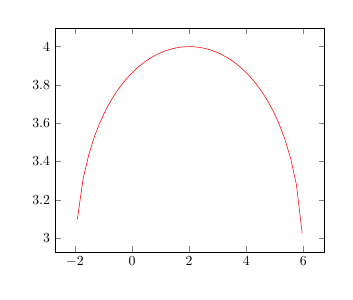
\begin{tikzpicture}[scale=0.5]
    \begin{axis}
      \addplot[color=red,domain=-10:10,samples=100]{sqrt(2+x)+sqrt(6-x)};
    \end{axis}
  \end{tikzpicture}
\end{center}

